\documentclass[a4paper, 12pt]{article}
\usepackage[utf8]{inputenc}
\usepackage[T1]{fontenc}
\usepackage{graphicx}
\usepackage{indentfirst}
\usepackage{hyperref}
\usepackage{float}
\usepackage{geometry}
\usepackage{graphicx}
\usepackage{svg}
\usepackage{tikz}
\usepackage{tikz-cd}
\usepackage{amsmath}
\geometry{left=3cm,right=3cm,top=2cm,bottom=2cm}

\title{%
  CarbonThink - Project Specifications \\
  \large RS6515 - Develop a decentralized application with blockchain technologies}
\author{William SIMON--VEZO}
\date{\today}

\begin{document}

\begin{figure}
\centering
\includesvg{carbonthink.svg}
\end{figure}

\maketitle

\begin{abstract}
This document explains the context, technical choices and requirements behind the CarbonThink project, developed as part of Alyra's Web 3 Developer training program.
\end{abstract}

\tableofcontents
\newpage

\section{Introduction}

\subsection{Context and Objectives}
\subsubsection{Project Context}
As part of the Alyra training "RS6515 - Developing a Decentralized Application with Blockchain Technologies" and to validate the skills necessary for certification, we, along with three other consultants from the same cohort, initiated the CarbonThink project.\\

CarbonThink addresses real-world needs: a relative of one of the consultants runs a company that assists farmers in decarbonization projects through bamboo planting, which entitles them to Carbon Credits. In exchange for the combined efforts of the company for project setup and support, the farmer for planting, and intermediary authorities for the official validation of decarbonization results, Carbon Credits are distributed. These Carbon Credits (1 credit = 1 ton of CO2) are then purchased by companies seeking to "offset" their carbon footprint, either out of philanthropy or due to legal obligations (as is the case for airlines).\\

The company's clients are now requesting a more traceable, accessible, verifiable, and immutable system: this is where Blockchain technology comes in. By registering the data of each project on the Blockchain (GPS coordinates, estimated tons of CO2, project duration, plant species planted, etc.), clients will be able to verify the origin and quality of the Carbon Credits they purchase.\\

In our project, we aim not only to enable clients to verify all this but also to offer a marketplace where these tokenized assets can be traded, always on the Blockchain. For clients, it is also important to prove to the authorities that the Carbon Credits they have purchased have indeed been validated for their annual offset report: hence, there is a need for a "burn" system for these tokenized Carbon Credits.

\subsubsection{Objectives}
The main objectives are multiple:

- Enable traceability, accessibility, verification, and immutability of data for clients;

- Partially eliminate dependence on authoritative registries (and their cost) by assuming this role as a company;

- Allow clients to purchase tokenized Carbon Credits;

- Enable clients to demonstrate to authorities that they have "used" these tokens to "offset" their emissions.

\subsubsection{Certification Requirements}
In order to obtain the certification, as a developer, I need to make sure that all those requirements are met at the end of the project:\\

C1. Write a requirements specification document describing the objectives, implementation methods, and features of a future decentralized application to conceptualize it and ensure its success.

C2. Develop a smart contract using a programming language suitable for blockchain technology to meet the functional needs of a decentralized application.

C3. Utilize a digital token (fungible or non-fungible) by using libraries and industry standards to implement a set of functionalities specific to a decentralized application.

C4. Identify security considerations and appropriate optimizations by analyzing the functionalities of a smart contract to prevent potential failures.

C5. Implement version control using continuous integration methods to ensure the viability of the application's development.

C6. Verify the resilience of a decentralized application by conducting functional tests to ensure its proper functioning for users.

C7. Develop computer code using a programming language suitable for web technologies to enable communication between a web and/or mobile interface and one or more smart contracts.

C8. Deploy a smart contract on a blockchain using a suitable development environment to make a decentralized application operational.

\subsection{Project Scope}

The scope of the project is:\\

- Create new carbon projects.

- Mint TCO2 tokens for the project holders.

- Store data in the Blockchain.

- Show data from the Blockchain in a front-end dapp.

- Build a Buy/Sell marketplace.

- Allow TCO2 tokens to be exchanged anywhere (OpenSea, Rarible, ...).

- Allow buyers to "burn" their TCO2 tokens in order to prove their "offset".

- Take a fee from the mints and put it into the Security Fund.

- Have "Royalties" on the token.

- Allow authorities and user to verify official documents.


\section{Needs Analysis}

\subsection{Functional Requirements}

As a team, we defined "User Stories" to break down tasks and clearly outline the necessary functionalities for each user, as well as to refine the details for each topic if needed.\\

The defined users are:\\

- The user (the buyer)

- CarbonThink (the administrator)

- The farmer (the project owner)

- The authority\\

For each task, we also set priorities in the development of each (P1 - "Main," P2 - "Secondary," P3 - "Nice to have").

\subsubsection{Functionalities}

\subsubsection{User Requirements}

Those are the Main user stories:\\

- As a User, I want to show a proof that I burned my tokens

- As a User, I want to burn my TCO2 tokens

- As a User, I want to see the info of a TCO2 token collection

- As a User, I want to see the info of a single TCO2 token

- As a User, I want to buy from the sell orders TCO2 tokens on the marketplace

- As a User, I want to have a view of a specific carbon project

- As a User, I want to have a view of all carbon projects

- As CarbonThink, I want to be able to create a new carbon project

- As CarbonThink, I want to Mint and transfer TCO2 tokens to a Project Holder

- As CarbonThink, I want to store official documents

- As CarbonThink, I want to manage the Security Funds

- As CarbonThink, I want a part of minted TCO2 tokens to go to the Security Fund

- As a Project Holder, I want a dashboard of my projects

- As a Project Holder, I want to see my projects

- As a Project Holder, I want to sell on the marketplace my TCO2 tokens \\

Those are the Secondary user stories:

- As a User, I want a dashboard of all my tokens (burned or not)

- As a User, I want to sell from the buy orders TCO2 tokens on the marketplace

- As CarbonThink, I want to receive royalties from marketplace transactions

- As an Authority, I want to verify official proof documents \\

Those are the "Nice to have" user stories:

- As a User, I want to define the token I will receive in exchange of my TCO2 tokens

- As CarbonThink, I want low fees on my read/writes from the blockchain

- As CarbonThink, I want to have a confirmation step for each request sent

- As CarbonThink, I want everyone to see how many tokens are generated / in exchange / burned so far

- As a Project Holder, I want to transfer my TCO2 tokens


\subsection{Non-Functional Requirements}
\subsubsection{Performance}

The response time of frontend calls must be fast enough to ensure that the use of the dapp is pleasant for users.\\

Regarding traffic load, the dapp must support a moderate flow of users. Since the backend is handled by the Blockchain and access providers, there should not be any issues on that side.\\

As CarbonThink will administrate the contracts, we want to reduce costs as much as possible and still have good performances on each read/write action. In order to do this, we will not use Ethereum as the main blockchain, as the gas fees are an issue with this many actions CarbonThink will have to execute in the long run. For this reason, we will use a layer 2 chain, transactions will be much cheaper as a result. As one of the requirements was allowing users to exchange their tokens anywhere easily, we will use the Base layer 2 blockchain, that is supported on OpenSea and other exchanges, and allows transactions directly with ETH tokens instead of a specific token created for the blockchain.

\subsubsection{Security}

The smart contract must only be able to be administered by CarbonThink.\\

Each user (buyer, CarbonThink, project holder) must be able to authenticate through their web3 wallets in order to perform actions on the Blockchain and/or the TCO2 tokens they own. A malicious actor shall not be able to attack the system with such an authentication required for accessing the dapp.\\

The data is not sensitive and must remain available to everyone.

\subsubsection{Compatibility}

Since we will be developing a frontend accessible on the internet for all browsers, compatibility with all major existing platforms is ensured.\\

Care must be taken regarding the use of the dapp on mobile devices, especially as mobile internet usage continues to become more widespread.

\subsubsection{Ergonomics and UI/UX}

The interface must be user-friendly enough for users to easily navigate the site structure. For this, we will use existing user-friendly frontend libraries for our dapp.

\section{Technical Specifications}

\subsection{Architecture}
\subsubsection{Architecture Diagram}

\begin{figure}[H]
    \centering
    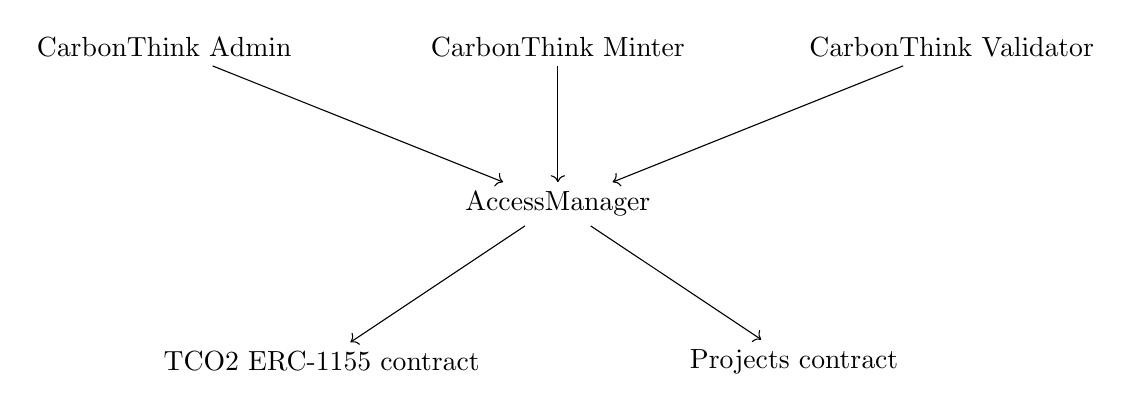
\begin{tikzpicture}
        \node (A) at (0,0) {CarbonThink Admin};
        \node (B) at (5,0) {CarbonThink Minter};
        \node (C) at (10,0) {CarbonThink Validator};
        \node (D) at (5,-2) {AccessManager};
        \node (E) at (2,-4) {TCO2 ERC-1155 contract};
        \node (F) at (8,-4) {Projects contract};
        \draw[->] (A) -- (D);
        \draw[->] (B) -- (D);
        \draw[->] (C) -- (D);
        \draw[->] (D) -- (E);
        \draw[->] (D) -- (F);
    \end{tikzpicture}
    \caption{CarbonThink management over the TCO2 token and projects with an AccessManager. Mint, project creation and validations go through a validation process in the AccessManager in order to avoid errors from CarbonThink.}
    \label{fig:carbonthink-accessmanager}
\end{figure}

\begin{figure}[H]
    \centering
    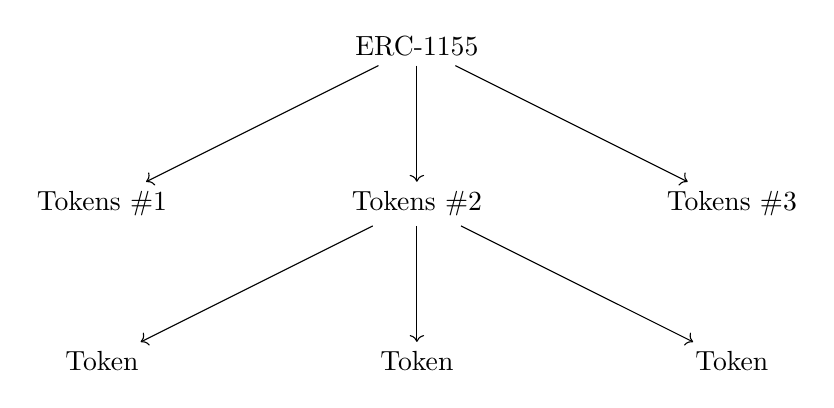
\begin{tikzpicture}
        \node (A) at (4,0) {ERC-1155};
        \node (B) at (0,-2) {Tokens \#1};
        \node (C) at (4,-2) {Tokens \#2};
        \node (D) at (8,-2) {Tokens \#3};
        \node (E) at (0,-4) {Token};
        \node (F) at (4,-4) {Token};
        \node (G) at (8,-4) {Token};
        \draw[->] (A) -- (B);
        \draw[->] (A) -- (C);
        \draw[->] (A) -- (D);
        \draw[->] (C) -- (E);
        \draw[->] (C) -- (F);
        \draw[->] (C) -- (G);
    \end{tikzpicture}
    \caption{ERC-1155 structure: each token is defined with on-chain metadata at the token collection level, with an amount of tokens which can be traded anywhere. ERC-1155 allows batch actions, whereas ERC-721 would have required to trade the NFT token by token, which would have been a pain point for the users. Each token type corresponds to a different project.}
    \label{fig:erc-1155}
\end{figure}

\begin{figure}[H]
    \centering
    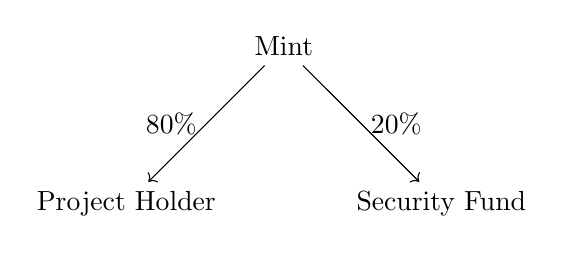
\begin{tikzpicture}
        \node (A) at (2,0) {Mint};
        \node (B) at (0,-2) {Project Holder};
        \node (C) at (4,-2) {Security Fund};
        \draw[->] (A) -- node[left] {80\%} (B);
        \draw[->] (A) -- node[right] {20\%} (C);
    \end{tikzpicture}
    \caption{Mint distribution. A part of the minted TCO2 tokens are given to the Security Fund in order to compensate the losses when some projects have issues. This works as an insurance.}
    \label{fig:mint-distribution}
\end{figure}

\begin{figure}[H]
    \centering
    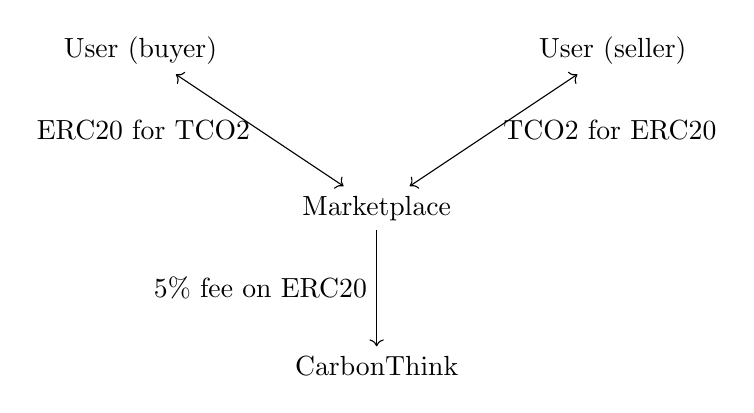
\begin{tikzpicture}
        \node (A) at (0,0) {User (buyer)};
        \node (B) at (6,0) {User (seller)};
        \node (C) at (3,-2) {Marketplace};
        \node (D) at (3,-4) {CarbonThink};
        \draw[<->] (A) -- node[left] {ERC20 for TCO2} (C);
        \draw[<->] (B) -- node[right] {TCO2 for ERC20} (C);
        \draw[->] (C) -- node[left] {5\% fee on ERC20} (D);
    \end{tikzpicture}
    \caption{Marketplace. The buyer will spend ERC20 tokens in order to buy TCO2 NFT tokens to the seller. A 5\% fee will be given to CarbonThink. A project holder can also sell their TCO2 tokens.}
    \label{fig:marketplace-fees}
\end{figure}

\subsubsection{Components}

ERC-1155 "TCO2" contract: defines all the rules for our TCO2 tokens. In this contract, we will write metadata on-chain at each token collection level in order to always have a trace of each token, instead of relying on IPFS like the majority of other projects do.\\

"Projects" contract: defines all the data (partially redundant with the metadata stored in each token collection metadata in the ERC-1155 "TCO2" contract). This contract will store the data that will be shown in our dapp frontend for our users to see.\\

AccessManager contract: here, we will define which addresses are able to execute admin actions on the TCO2 token (such as the "mint" function) or on the Projects contract (such as "createProject" function). Those actions are put into a time lock until the validator approves each of them individually.\\

Marketplace contract: we will also create a mini-marketplace for our users to buy and sell TCO2 tokens. Note that as we used the ERC-1155 standard, those NFT tokens can we exchanged anywhere, in places such as OpenSea or Rarible.

\subsubsection{Data to store}

As we will write information about all the CarbonThink projects, we have to define which data is interesting for the users to look. In order to keep track of each TCO2 token minted specifically for each project, some of these data will be stored as metadata in the ERC-1155 contract at the token collection level.\\

Project Data:\\

- Unique project identifier

- Project name

- Project location

- Project geolocation

- Project area

- Project launch date

- Cultivation methods

- Carbon Credits Data

- Carbon capture capacity

- Program duration (number of years)

- Total quantity of carbon credits for the program

- CO2 emissions schedule

- Audit and Validation Data

- Cultivation protocol

- Initial report

- Audit reports

- Management and Monitoring Data

- Project status

- Periodic updates

- Photographs and images


\subsection{Technologies Used}
\subsubsection{Programming Languages}

All the technologies seen and used during Alyra's training in the past few months will be reused, in order to master those and confirm our abilities to use industry standard tools.\\

For the smart contract, we will use Solidity as the main programming language. Unit tests will be written with Hardhat in Typescript. Hardhat will also be used for the deployment of our project, and for internal tests on the Hardhat local blockchain. OpenZeppelin contracts will also be a must have in order to develop our own contracts.\\

For the frontend part, we will use NextJS with React and use Typescript as the main language.

\subsubsection{Frameworks and Libraries}

Frontend:

- React

- NextJS

- TailwindCSS

- Shadcn

- ConnectKit

- Wagmi\\

Backend \& CI/CD:

- Hardhat

- Vercel

- Prettier

- Cspell

- Solhint

- Slither


\subsubsection{Infrastructure}

- IPFS for file storage (official documents).

- Base Layer 2 blockchain on Ethereum.

- Vercel as the host for our dapp.


\section{Testing}

Unit tests will be written with a 100\% code coverage over all the Solidity contracts in order to make sure that nothing will break during our deployment to production. Those Unit Tests will be written using Hardhat and Chai.\\

Some frontend integration / unit tests could also be written if we have enough time to do so.

In order to maintain the project easily, Github actions have been set in order to check that everything is working nicely at each push on the repository (backend-lint, frontend-lint, backend-test-hardhat, slither check and finally codespell check). Git hooks have been set too, in order to check locally before any push that some quality requirements are met, such as a valid lint for each file and valid unit tests.

A ".vscode" config folder also has been set in order to keep the same configuration for each developer in the project. In this project, only one developer is actively working on it, but it's still good practices.

\section{Development Plan}

\subsection{Schedule}
\subsubsection{Project Phases}

First week: full analysis with the team about the needs of the project.\\

Second week: develop all the needed smart contracts and complete the unit tests coverage to 100\%. Also, generate NatSpecs and documentation accordingly.\\

Third and last week: develop the frontend, do as much bug-fixing as possible in order to have a nice dapp, both styled and usable.\\

Fortunately, all the work done during Alyra's training in the past few months will be a nice start for the project and will be reused.

\subsubsection{Timeline}

The project must be complete and delivered before Sunday the 14th in the evening.\\

Finishing the project a few days earlier would be nice for the team in order for everyone to see what have been implemented in the allotted time.

\subsection{Team}

Christophe DEBRAS, consulting.\\

Philippe MARCHAND, consulting.\\

Virgile GRANDJEAN, consulting.\\

William SIMON--VEZO, development.

\appendix
\section{References}

\href{https://nextjs.org/}{NextJS}.\\

\href{https://vercel.com/varadiells-projects}{Vercel}.\\

\href{https://fr.react.dev/}{React}.\\

\href{https://tailwindcss.com/}{TailwindCSS}.\\

\href{https://ui.shadcn.com/}{Shadcn}.\\

\href{https://docs.family.co/connectkit}{ConnectKit}.\\

\href{https://wagmi.sh/}{Wagmi}.\\

\href{https://hardhat.org/}{Hardhat}.\\

\href{https://prettier.io/}{Prettier}.\\

\href{https://cspell.org/}{Cspell}.\\

\href{https://github.com/protofire/solhint}{Solhint}.\\

\href{https://github.com/crytic/slither}{Slither}.\\

\href{https://resources.github.com/devops/ci-cd/}{Github CI/CD}.\\

\href{https://ipfs.tech/}{IPFS}.\\

\href{https://github.com/OpenZeppelin/openzeppelin-contracts}{Open Zeppelin contracts}.\\

\href{https://ethereum.org/fr/developers/docs/standards/tokens/erc-1155/}{ERC-1155}.\\

\href{https://www.base.org/}{Base Layer 2}.\\

\href{https://www.climateimpact.com/services-projects/carbon-credits-explained-what-they-are-and-how-they-work/}{Carbon Credits explained}.\\

\end{document}
